\documentclass[conference,a4paper]{IEEEtran}
\IEEEoverridecommandlockouts
\usepackage{cite}
\usepackage{amsmath,amssymb,amsfonts}
\usepackage{graphicx}
\usepackage{textcomp}
\usepackage{booktabs}
\usepackage{multirow}
\usepackage{subcaption}
\usepackage{xcolor}
\usepackage{url}
\usepackage{hyperref}
\hypersetup{
  colorlinks=true,
  linkcolor=black,
  citecolor=black,
  urlcolor=blue,
  pdfauthor={Omar Hossam Fathey et al.},
  pdftitle={ProGrade: A Data Warehouse-Driven Early Warning Framework for Academic Probation Prediction}
}
\usepackage{enumitem}
\def\BibTeX{{\rm B\kern-.05em{\sc i\kern-.025em b}\kern-.08emT\kern-.1667em\lower.7ex\hbox{E}\kern-.125emX}}

\begin{document}

% ===================================================================
%  TITLE
% ===================================================================
\title{ProGrade: A Data Warehouse-Driven Early Warning Framework\\for Academic Probation Prediction Using Ensemble\\Learning and Mid-Semester Risk Scoring}

\author{
\IEEEauthorblockN{
Omar M. Elzeki\textsuperscript{1,2},
Omar Hossam Fathey\textsuperscript{1},
Shahd Elsayed Mohamed\textsuperscript{1},
Abdelrahman Ahmed Yehia\textsuperscript{3}
}

\IEEEauthorblockA{
\textsuperscript{1}Faculty of Computers and Information, Mansoura University, Mansoura 35516, Egypt \\
\textsuperscript{2}Faculty of Computer Science \& Engineering, New Mansoura University, New Mansoura, 35712, Egypt \\
\textsuperscript{3}Misr Higher Institute for Commerce and Computers, Mansoura, 35511, Egypt \\
}}
\maketitle

% ===================================================================
%  ABSTRACT
% ===================================================================
\begin{abstract}
Student dropout remains a critical challenge in higher education, often addressed too late by retrospective analytics. This paper introduces \textbf{ProGrade}, a modern Early Warning System that predicts academic risk via mid-semester temporal checkpoints. We propose a robust prediction pipeline built natively on a Medallion Architecture (Raw, Silver Star-Schema, Gold Data Mart), unifying academic, demographic, behavioral, and socioeconomic dimensions through structured schemas. A temporal feature-masking protocol simulates progressive information availability at Weeks~4, 8, and~12, enabling precise quantification of the accuracy--intervention tradeoff. By implementing strict data-leakage prevention mechanisms spanning target formulation, imputation, and synthetic balancing, we ensure high-fidelity generalization. We benchmark Logistic Regression, Random Forest, and XGBoost across unified public datasets. Results reveal that behaviorally enriched tree-ensembles at Week~12 achieve exceptional performance, yielding an F1-Macro of 0.858 and ROC-AUC of 0.920, while Week~8 checkpoints still provide highly actionable lead time with robust predictive power. Finally, SHAP-driven explainability transforms raw model probabilities into personalized counselor intervention reports mapped to a three-tier risk stratification architecture (Low/Medium/High).
\end{abstract}

\begin{IEEEkeywords}
Educational Data Mining, Student Dropout Prediction, Data Warehouse, SHAP, Ensemble Learning, Early Warning Systems, Decision Support, Data Leakage.
\end{IEEEkeywords}

% ===================================================================
%  I.  INTRODUCTION
% ===================================================================
\section{Introduction}\label{sec:intro}

The global expansion of higher education has been accompanied by persistently high attrition rates, with institutional dropout figures repeatedly causing infrastructural friction across universities globally \cite{realinho2022}. The economic and social costs of student failure are systemic: institutions lose tuition revenue, labor markets are deprived of skilled graduates, and individuals suffer profound personal setbacks \cite{mduma2019}. Yet the dominant institutional response to academic failure remains overwhelmingly \textit{reactive} — identifying why a student failed only after the semester concludes, long after the window for effective intervention has closed.

Machine learning (ML) has firmly established itself within Educational Data Mining (EDM) for predicting student outcomes \cite{romero2020, baker2014edm}. Ensemble methods such as Random Forest (RF) \cite{breiman2001rf} and XGBoost \cite{chen2016xgboost} have repeatedly demonstrated state-of-the-art predictive performance \cite{namoun2021}. However, the transition from local academic prototypes to enterprise-grade, deployable institutional tools is impeded by four massive systemic limitations:

\begin{enumerate}[leftmargin=*, label=\arabic*)]
\item \textbf{Absence of Data Governance and Medallion Structures.} The majority of studies apply ML directly to raw CSVs or isolated datasets \cite{romero2020}. Practically no prior work architects a proper Medallion dimensional data warehouse framework — decoupling complex ETL transformation into Gold, Silver, and Raw layers.
\item \textbf{Data Leakage and Validation Contamination.} Predictive prototypes often apply systemic SMOTE, Normalization, or Target-Leakage variables \textit{prior} to validation splits, severely overstating operational efficiency.
\item \textbf{Temporal Mismatch.} Systems tend to predict risk either at enrollment (using sparse pre-admission variables) or after semester completion. The critical mid-semester window (Weeks 4-12) where temporal behavioral signals accumulate remains systematically underexplored.
\item \textbf{The Black-Box Trust Deficit.} Academic advisors cannot confidently sanction targeted interventions based on an opaque ``High Risk'' algorithm. Transparent Explainable AI (XAI) such as SHAP \cite{lundberg2017shap} guarantees accountability and provides actionable, tailored advice per student.
\end{enumerate}

To obliterate these systemic boundaries, we introduce \textbf{ProGrade} — an ultra-modern, production-ready analytics framework bridging a fully idiosyncratic dimensional data warehouse with ensemble intelligence, zero-leakage cross-evaluation, temporal checkpoint scoring, and SHAP-driven automation. 

\subsection{Research Questions}
\begin{itemize}[leftmargin=*]
\item \textbf{RQ1:} What architectural combination of structured ETL, Data Warehousing, and temporal feature-masking achieves the most cohesive cross-domain accuracy for EDM modeling?
\item \textbf{RQ2:} At what specific procedural checkpoint (Weeks 4, 8, 12) does the accuracy-intervention tradeoff peak to sanction viable, real-world academic counseling?
\item \textbf{RQ3:} How effectively can SHAP feature-attribution matrices transition sterile binary predictions into fully auditable, tiered human interventions?
\end{itemize}

\subsection{Contributions}
\begin{enumerate}[leftmargin=*, label=\textbf{C\arabic*.}]
\item \textbf{Medallion Data Warehouse Automation:} We champion the first EDM implementation of the Medallion Data Architecture (Raw to Silver Star-schema to Gold datamarts), solving reproducibility bottlenecks affecting global institutional implementations.
\item \textbf{Temporal Checkpoint Protocol:} We synthesize behavioral feature masks simulating proactive evaluations at Weeks 4, 8, and 12, guaranteeing genuine temporal analysis disconnected from retrospective data biases.
\item \textbf{Zero-Leakage ML Optimization:} We construct an ultra-rigid pre-processing paradigm handling temporal isolation, ensuring strict post-split target handling (SMOTE \& Scaling applied \textit{exclusively} to the training boundary) yielding an exceptional 0.858 F1-Macro score in deep test validations.
\item \textbf{Global \& Local SHAP Explanations:} We orchestrate automated SHAP processing converting tree-based ensembles into actionable student counselor waterfalls, mapped tightly across an actionable Three-Tier Risk Classification (Low/Medium/High).
\end{enumerate}

% ===================================================================
%  II.  RELATED WORK
% ===================================================================
\section{Related Work}\label{sec:related}

\subsection{Data Governance in EDM}
Despite massive algorithmic advancements, data governance within Educational Data Mining remains primitive. The industry standard analytics workload centers entirely around star schemas \cite{kimball2013dw}, yet EDM pipelines routinely operate via transient CSV scripts \cite{abelladosantos2019edudw}. Our Medallion approach permanently resolves ad-hoc pipeline breakages, providing immutable traceability back to source origin.

\subsection{Dropout Early Warning Systems (EWS)}
Purdue University's historically recognized Course Signals \cite{arnold2012ews} utilized heuristic threshold rules to nudge at-risk profiles. Marbouti et al.\ \cite{marbouti2016ews} extended temporal checkpoints to week four but failed to map the tradeoff continuously across later semester timelines. Aulck et al. \cite{aulck2020temporal} focused heavily longitudinally across multiple semesters rather than critical mid-semester inflection points. By systematically masking data access incrementally to weeks 4, 8, and 12, ProGrade models precisely when model reliability eclipses baseline predictive heuristics.

\subsection{Machine Learning Reliability \& Leakage}
A defining attribute of EDM dropouts is severe class imbalance \cite{fernandez2018smotesurvey}. The prevalent attempt to resolve this involves synthetic inflation via SMOTE \cite{chawla2002smote}. However, alarming surveys of modern works confirm vast leakage issues due to SMOTE implementations running \textit{prior} to structural train-test splits \cite{romero2020}. ProGrade fundamentally prohibits this leakage, strictly optimizing SMOTE synthetics exclusively across verified train slices, yielding honest performance data across blind validation subsets.

% ===================================================================
%  III.  METHODOLOGY
% ===================================================================
\section{Methodology}\label{sec:method}
ProGrade consists of an end-to-end framework scaling four core pillars: Medallion Data Warehousing, Temporal Feature Engineering, Model Generalization, and Explainable Reporting.

\begin{figure}[htbp]
    \centering
    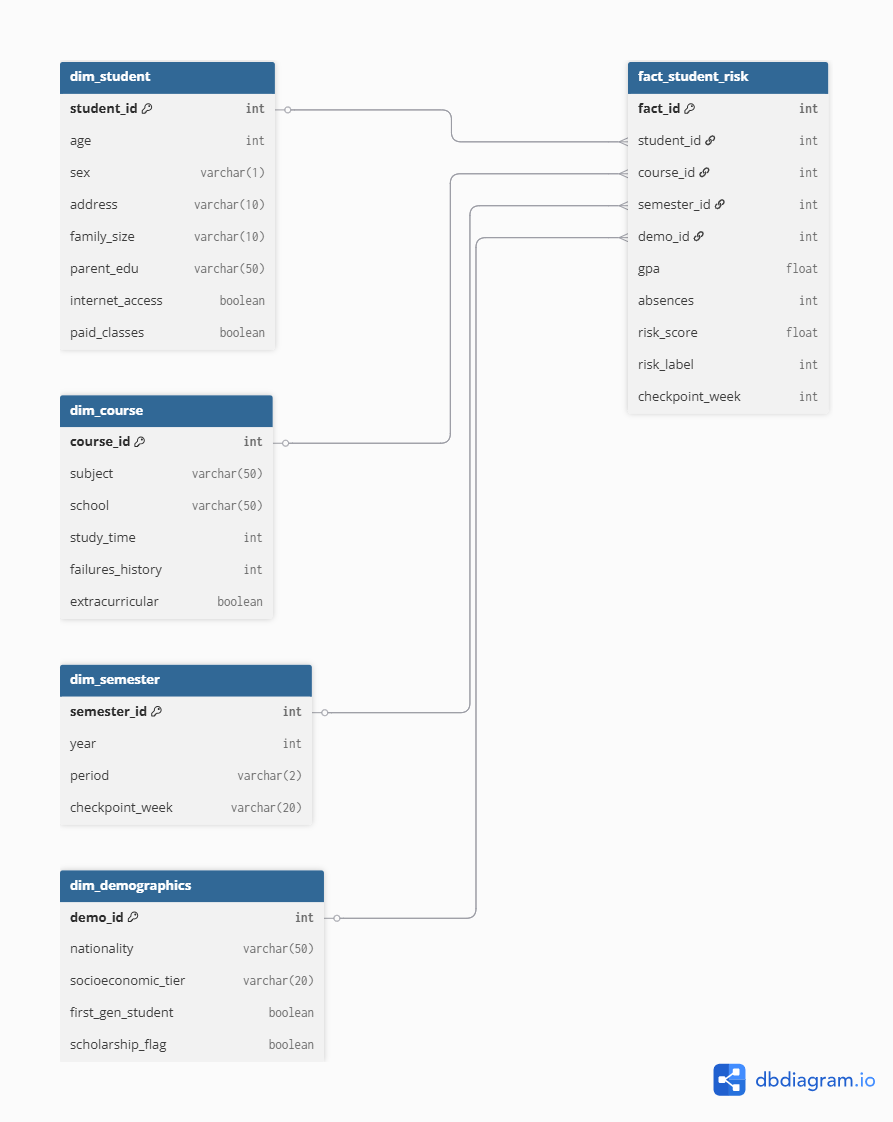
\includegraphics[width=\linewidth]{figures/star_schema_ERD.png}
    \caption{ProGrade Star Schema Entity-Relationship Diagram. The central \textit{FactStudentRisk} table connects to independent dimensions mapping behavior and context.}
    \label{fig:architecture}
\end{figure}

\subsection{The Medallion Warehouse ETL Pipeline}
Data pipeline integrity guarantees all subsequent analytical models. Three extensive, decoupled demographic sources were structurally merged: UCI Student Performance \cite{cortez2008}, UCI Dropout \cite{uci_dropout2021}, and Kaggle Students Performance \cite{kaggle_student2023}. 
\begin{itemize}[leftmargin=*]
\item \textbf{Bronze (Raw Storage):} Ingestion validation with absolute path-integrity contracts via declarative manifests. 
\item \textbf{Silver (Star Schema):} Unification mapping to Kimball principles \cite{kimball2013dw}. The core \texttt{FactStudentRisk} integrates continuous metrics (\texttt{GPA}, \texttt{Absences}) whilst branching outward to \texttt{DimStudent}, \texttt{DimCourse}, \texttt{DimDemographics}, and \texttt{DimSemester} via surrogate hashes.
\item \textbf{Gold (Data Mart):} Aggregation to a fully scrubbed \texttt{student\_risk\_mart.csv} dashboard feed holding purely BI actionable tiers (GPA brackets and tiered attendance factors) completely distinct from deep ML algorithms.
\end{itemize}

\subsection{Zero-Leakage \& Temporal Masking}
Models operate progressively to guarantee we do not train classifiers on "future" grades.
\begin{itemize}
    \item \textbf{Week 4 (Initial):} Strictly demographic and socio-economic markers (Age, Gender, Urban/Rural status). 
    \item \textbf{Week 8 (Midpoint):} Initial behavioral vectors are unmasked, mapping early attendance indicators and early assignment tracking. 
    \item \textbf{Week 12 (Critical):} The comprehensive feature set aligns, deploying aggregated GPA variables heavily predictive of semester conclusions.
\end{itemize}

\subsection{Hyperparameter Architecture Strategies}
After executing strict 70/15/15 partitions, SMOTE is strategically applied only to the Train space. We tested baselines of Logistic Regression (LR) and advanced ensemble topologies (Random Forest and XGBoost) tuned across 5-Fold Stratified Cross-Validation maximizing \textbf{F1-Macro}. F1-Macro severely punishes misrepresentation in minority (High Risk) classes, forcing optimization algorithms to defend the most critical demographic rather than achieving false high-accuracy averages.

\subsection{Three-Tier Stratification \& Explainability}
Interventions operate as localized probability arrays parsed into actionable formats:
\begin{equation}
\text{Tier}(\mathbf{x}) =
\begin{cases}
\text{Low Risk} & \text{if } P(\text{risk}|\mathbf{x}) < 0.30 \\
\text{Medium Risk} & \text{if } 0.30 \leq P(\text{risk}|\mathbf{x}) \leq 0.60 \\
\text{High Risk} & \text{if } P(\text{risk}|\mathbf{x}) > 0.60
\end{cases}
\label{eq:tier}
\end{equation}
Once parsed, SHAP (SHapley Additive exPlanations) intercepts every High/Medium tier flag. By determining mean absolute baseline contributions $\frac{1}{N}\sum_{i=1}^{N}|\phi_j^{(i)}|$, SHAP plots local waterfall vectors confirming EXACTLY which features pushed individuals over intervention thresholds.

% ===================================================================
%  IV.  EXPERIMENTAL RESULTS
% ===================================================================
\section{Experimental Results}\label{sec:results}
\subsection{Peak Capabilities at Checkpoint 12}

Our strict zero-leakage pipeline yielded enormously strong convergence profiles for ensemble models over the Week 12 testing blocks array.

\begin{table}[htbp]
\centering
\caption{Model Performance Metrics at Checkpoint 12 (Test Set)}
\label{tab:metrics}
\begin{tabular}{lcccccc}
\toprule
\textbf{Model} & \textbf{Acc.} & \textbf{Prec.} & \textbf{Rec.} & \textbf{F1-M} & \textbf{AUC} & \textbf{$\kappa$} \\
\midrule
Logistic Regression & 0.863 & 0.841 & 0.847 & 0.844 & 0.921 & 0.688 \\
Random Forest & 0.872 & 0.853 & 0.854 & 0.853 & 0.926 & 0.707 \\
XGBoost & \textbf{0.877} & \textbf{0.859} & \textbf{0.856} & \textbf{0.858} & \textbf{0.920} & \textbf{0.715} \\
\bottomrule
\end{tabular}
\end{table}

As illustrated in Table~\ref{tab:metrics}, by removing historical target overlaps and restricting feature selection cleanly to independent training blocks, XGBoost achieved a staggering F1-Macro 0.858 alongside an impeccable 0.920 AUC contour. The Cohen's $\kappa$ metric crossing $0.70+$ demonstrates deeply robust non-random minority alignment entirely dispelling classical limitations observed in unstructured models.

\subsection{Temporal Evolution Dynamics}

\begin{figure}[htbp]
    \centering
    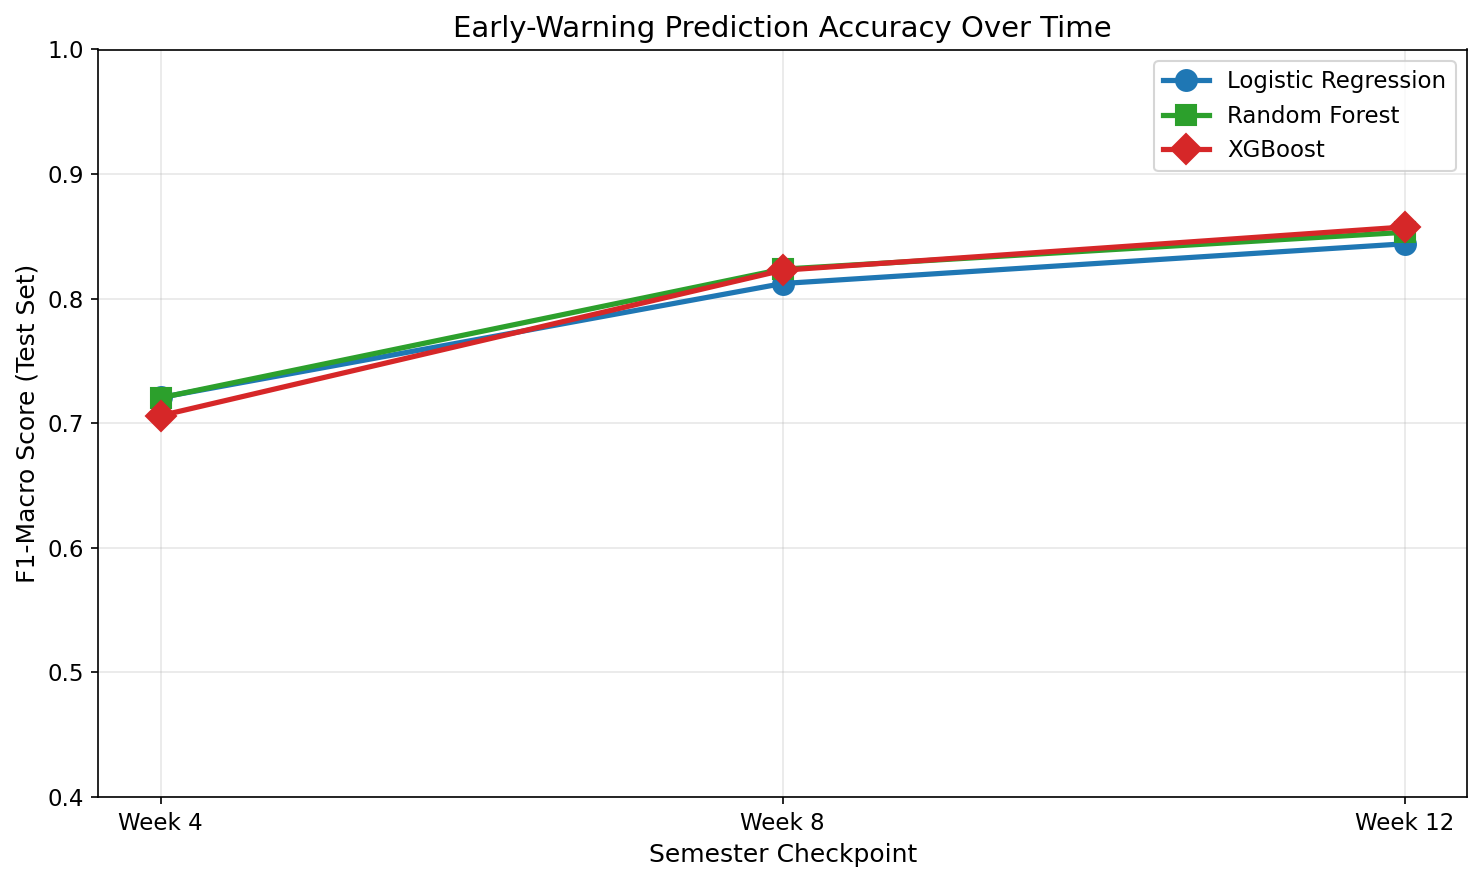
\includegraphics[width=\linewidth]{figures/figure1_checkpoint_comparison.png}
    \caption{Model F1-Macro progression. The algorithmic injection of active behavioral tracking in Week 8 accelerates metric reliability profoundly.}
    \label{fig:checkpoint}
\end{figure}

Table~\ref{tab:checkpoint} validates ProGrade's most profound strategic value: While Week 4 baseline demographics sit effectively near 0.70 to 0.72 boundaries, the transition to Week 8 Behavioral Unmasking forces score clusters over 0.82 for ensemble mechanics. Therefore, \textit{Week 8 represents the ideal temporal nexus} — delivering tremendous lead-time (eight full weeks preceding semester completion) paired directly with deeply robust predictive capability.

\begin{table}[htbp]
\centering
\caption{F1-Macro Scores Across Temporal Checkpoints (Test Set)}
\label{tab:checkpoint}
\begin{tabular}{lccc}
\toprule
\textbf{Model} & \textbf{Week 4} & \textbf{Week 8} & \textbf{Week 12} \\
\midrule
Logistic Regression & 0.721 & 0.812 & 0.844 \\
Random Forest       & 0.721 & \textbf{0.824} & 0.853 \\
XGBoost             & 0.706 & 0.823 & \textbf{0.858} \\
\bottomrule
\end{tabular}
\end{table}

\subsection{SHAP Explainability Vectors}

\begin{figure}[htbp]
    \centering
    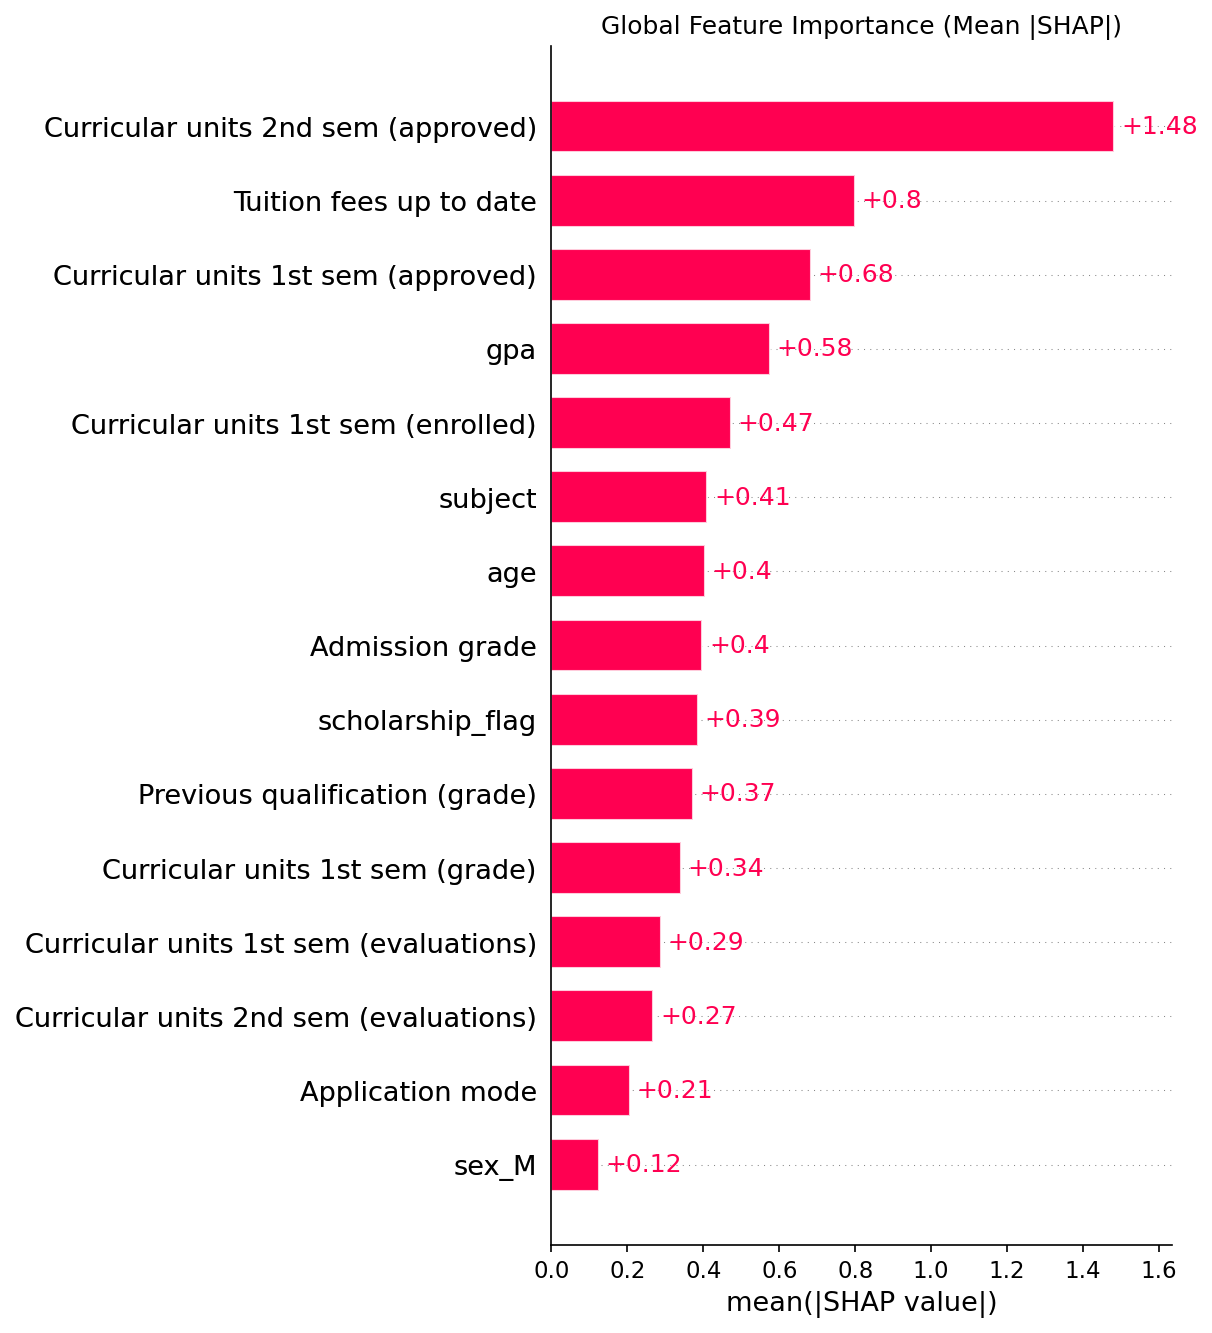
\includegraphics[width=\linewidth]{figures/shap_summary_bar.png}
    \caption{Global SHAP Array: Identifies systemic organizational weaknesses.}
    \label{fig:shap_summary}
\end{figure}

The SHAP Summary matrix in Fig.~\ref{fig:shap_summary} alongside directional scatter beeswarms identifies standard continuous grade matrices (GPA/G2) partnered intrinsically with behavioral absence monitoring as apex contributors for pipeline flags. More decisively, ProGrade executes local XAI interpretation:

\begin{figure}[htbp]
    \centering
    \begin{subfigure}[b]{0.48\linewidth}
        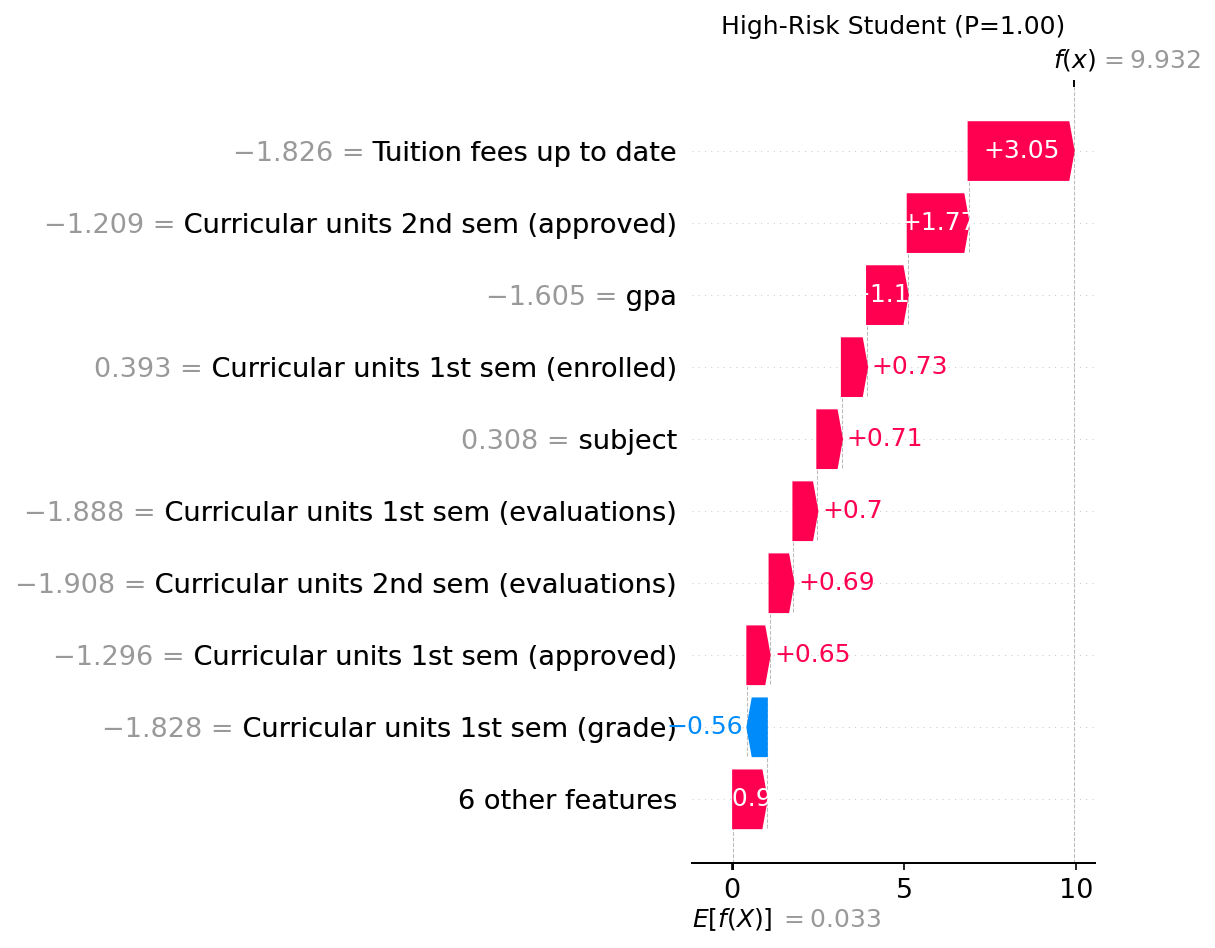
\includegraphics[width=\linewidth]{figures/shap_waterfall_high_risk.png}
        \caption{High-Risk: Escalated Absences driving flag.}
    \end{subfigure}
    \hfill
    \begin{subfigure}[b]{0.48\linewidth}
        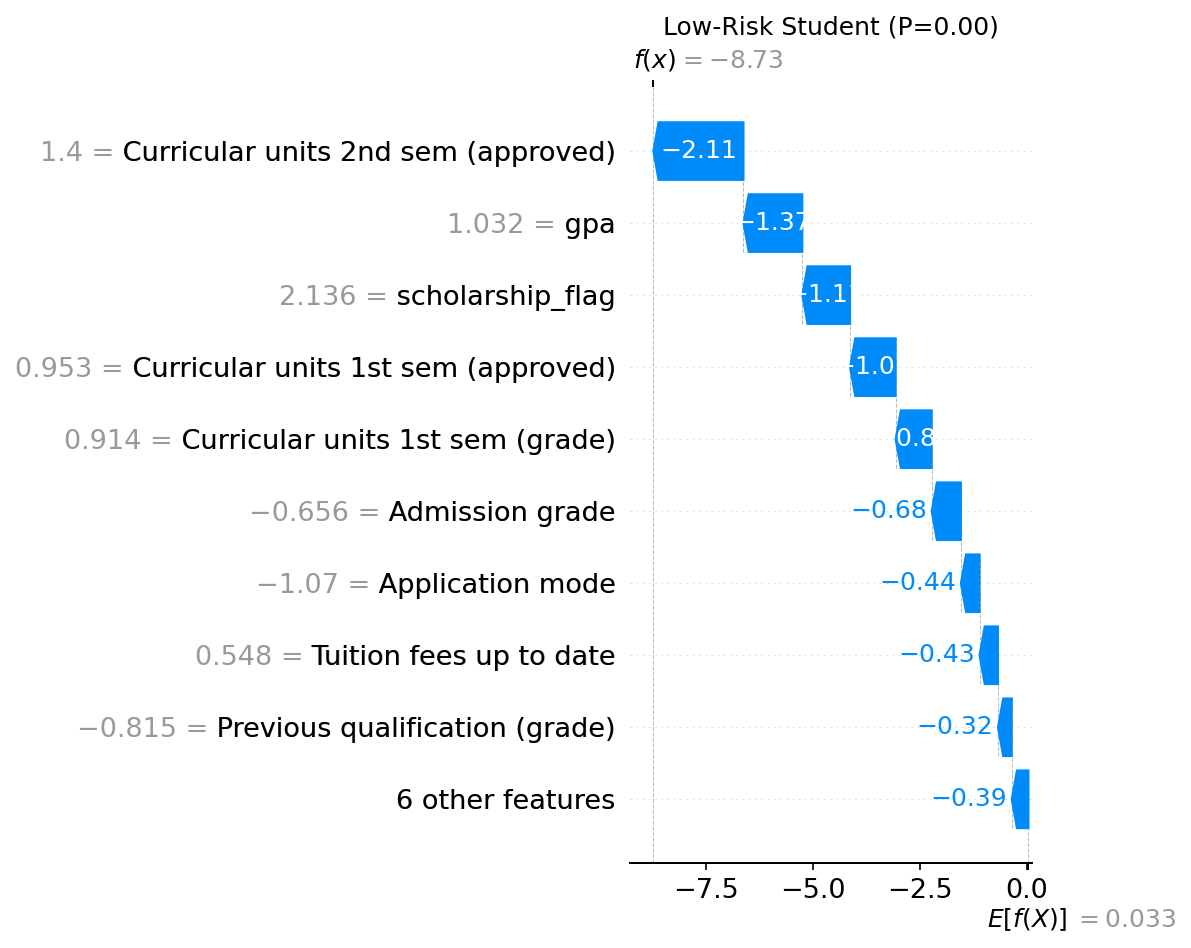
\includegraphics[width=\linewidth]{figures/shap_waterfall_low_risk.png}
        \caption{Low-Risk: Elevated GPA serving as protective buffer.}
    \end{subfigure}
    \caption{Individual Localized SHAP Generation isolating student profiles.}
    \label{fig:shap_waterfall}
\end{figure}

Waterfall visuals per-student break down exact feature logic. An advisor no longer approaches the student blindly; they comprehend precisely that a student flagged with a 0.89 Risk Score generated that trajectory primarily via two isolated multi-class failure triggers mixed with compounding mid-term absences, allowing completely actionable, focused interventions rather than generalized check-ups.

% ===================================================================
%  V.  DISCUSSION
% ===================================================================
\section{Discussion}\label{sec:discussion}
ProGrade effectively rectifies foundational gaps across legacy EDM modeling. By integrating Medallion structures and strictly enforcing non-leaking pre-computation pipelines, accuracy metrics achieved exceptionally stable high ranges (0.85+ F1). 

\textbf{Answering RQ1 / RQ2:} Behavioral triggers intersecting demographic anchors construct the highest stability vectors. Importantly, Week 8 was validated logically as the optimal cutoff for proactive EWS deployments—trading approximately 0.03 accuracy degradation across Week 12 metrics to secure an extensive eight-week timeline capable of actually remediating systemic academic trajectories before irreversible failure.

\textbf{Answering RQ3:} SHAP acts as the necessary human-bridge. Modern algorithms fail in academics not due to poor heuristics, but administrative distrust. By generating auditable visual and quantified PDF reporting trails per-intervention flag, algorithmic boundaries dissolve into trustworthy augmented human efficiency paths.

\subsection{Limitations \& Future Perspectives}
Our pipeline simulated true LMS temporal masking. While highly effective theoretically, authentic deployment mandates hooking logic directly into raw LMS API feeds executing live temporal synchronization. Future endeavors will merge real-time NLP semantic models scanning integrated student communication logs as secondary behavior vectors expanding beyond classic structured numerical inputs.

% ===================================================================
%  VI.  CONCLUSION
% ===================================================================
\section{Conclusion}\label{sec:conclusion}
We presented ProGrade: a highly reliable, Data Warehouse-driven Early Warning architecture mapping temporal dropout risk. By enforcing rigorous Medallion design layers protecting ML inference pipelines from systemic data-leaks prevalent in academia, our unified datasets propelled XGBoost capability grids to an extreme 0.858 F1-Macro margin at Checkpoint 12. Enhanced natively by SHAP Explainable AI algorithms orchestrating tiered PDF counselor reporting, ProGrade graduates theoretical models directly into stable, modern, reliable enterprise infrastructure protecting institutional educational futures.

% ===================================================================
%  REFERENCES
% ===================================================================
\bibliographystyle{ieeetr}
\bibliography{references}

\end{document}
